\newcounter{proposalRefCount}
% [1] 表示有 1 个参数
% [1] (第二个) 表示该参数可选，默认值为 1
\newcommand{\proposalRef}[1][1]{%
    \newcount\i% 定义一个局部循环变量
    \i=1%
    [\loop\ifnum\i<#1% 开始循环，次数为参数 #1
        \stepcounter{proposalRefCount}% 计数器自增 1
        \theproposalRefCount, % 显示当前数字
        \advance\i by 1% 循环变量 +1
    \repeat%
    \stepcounter{proposalRefCount}% 计数器自增 1
    \theproposalRefCount]% 显示当前数字
}

\usepackage{caption}

% 1. 研究现状、水平、趋势
\researchStatus{
    站点可靠性工程 (Site Reliability Engineering, SRE) 是一套原则和实践，旨在创建可扩展且高度可靠的软件系统。它起源于 Google，将软件工程的方法应用于基础设施和运维问题。SRE 的核心任务包括但不限于：
    \begin{itemize}
    \item 故障检测 (Detection): 通过监控日志、指标等遥测数据，及时发现系统出现的异常。
    \item 故障定位 (Localization): 确定故障发生的具体组件或模块。
    \item 根本原因分析 (Root Cause Analysis, RCA): 找出导致故障的根本原因，如软件 Bug、配置错误等。
    \item 故障缓解 (Mitigation): 采取措施阻止故障蔓延、恢复服务，例如重启服务、回滚代码、切换流量等。
    \end{itemize}
    现代云系统规模庞大、复杂且动态，导致故障频发，在这一背景下传统 SRE 方法面临着如下这些问题和挑战：\proposalRef

    \begin{enumerate}[label=\arabic*)]
    \item{
        严重依赖于人类工程师手动收集和分析各种数据源，如日志、指标、跟踪和事件工单。这种手动过程不仅费力、容易出错，而且在面对信息过少或信息过载时尤其具有挑战性。相关信息可能被埋在海量数据中，导致人类工程师难以快速找到关键线索。这样的人工方式响应速度慢、成本高，已无法跟上现代云系统的规模和故障频率。
    }
    \item{
        故障排查指南 (Troubleshooting Guides, TSGs) 和标准作业程序 (Standard Operating Procedure, SOP) 是运维工程师为了标准化和加速故障排查而创建的基于经验总结的最佳实践，但它们也有如下局限：
        \begin{itemize}
        \item 手动数据集成: 仍需人类工程师手动从不同来源收集数据，耗时且易错。
        \item 信息过时: TSG 和 SOP 作为静态文档，难以跟上云系统快速演进的步伐，导致其内容可能过时或不完整。
        \item 细节不足和覆盖范围有限: TSG 和 SOP 通常提供高层级指导，缺乏细节，且可能无法覆盖所有复杂情境或新出现的事件类型。
        \end{itemize}
    }
    \end{enumerate}
    AIOps (Artificial Intelligence for IT Operations)\proposalRef 正是为了解决这些挑战而诞生，它将人工智能 (AI) 技术应用于 IT 运维 (IT Operations) 领域，通过利用大数据、机器学习和高级分析来自动化和增强对 IT 基础设施的监控、管理和问题解决能力。AIOps 以往的技术演进可以大致分为以下几个阶段：
    \begin{enumerate}[label=\roman*)]
    \item 纯手动运维: 工程师手动登录服务器，查看日志，执行命令。效率低下，极易出错。
    \item 脚本化自动化: 工程师编写运维脚本（如 Shell, Python脚本）来自动化重复性任务。脚本是固化的，难以适应动态变化。
    \item 辅助性 AI 工具: AI/ML 模型开始被用于分析海量遥测数据，为人类提供洞察和建议。
    \end{enumerate}
    LLM Agent 作为一种新兴的 AI 技术，展示了在复杂任务中自主决策和执行的潜力。传统方法通常基于特定指标或历史模式，泛化能力有限，难以处理新类型事件。利用 LLM 的逻辑推理和泛化能力，能够进行更全面的分析，有望革新 SRE 实践。但它们缺乏领域特定知识 (domain-specific knowledge)，尤其是在云事件管理等专业领域。前人已探索了\textbf{微调} (fine-tuning) LLM 适应 SRE 任务的方法\proposalRef 和引入\textbf{多智能体投票机制}的方法\proposalRef，提升了故障诊断的准确率，取得了一定成效。然而，这些方法仍然仅限于数据集上获得更好的成绩，难以落地到实际场景。尤其是微调的方法仍然存在成本高昂、需要大量训练样本、难以持续更新以适应事件演变以及容易产生幻觉 (hallucinated) 结果等问题。

    当前的 AIOps 正趋向于赋予 Agent 决策和执行的能力，使其能够自主解决问题。STRATUS 的工作\proposalRef 是最为前沿的代表，成功验证了\textbf{多智能体协作}架构下的 SRE 端到端实践可行性。
}

% 2. 研究目的和意义
\researchSignificance{
    推动大语言模型智能体（LLM Agent）在站点可靠性工程（SRE）领域的深度实践，其核心挑战已超越了在通用基准数据集上追求单纯的异常检测准确率或根因分析覆盖率。真实世界的 IT 系统具有高度的异构性与动态性，这要求智能体必须具备从“通用泛化”向“系统特化”转化的能力。

    本研究提出了一种基于多智能体协作的自主演练框架。在该框架下，LLM Agent 不再被动地等待故障发生，而是以主动探索的方式接入新系统环境：利用现有的混沌工程工具计划地注入模拟故障，智能体能够建立起对特定拓扑结构和指标关联的直观感知。在这一过程中，多个智能体分工协作，模拟从实时监控、故障精准定位、深层根因追溯到自动化修复缓解的全生命周期任务，在实战演练中验证其决策链条的可靠性。

    同时，本研究首次在 AIOps 中引入了上下文的\textbf{自适应}（Self-Evolve）演化机制。在每一次端到端工作流闭环后，系统会启动深度回顾程序，对推理轨迹的合理性、动作执行的有效性以及最终的反馈结果进行自动化审计。通过提取成功经验与复盘失败教训，智能体能够将这些碎片化的实践转化为结构化的系统知识库。这种基于反馈的持续学习模式，使 LLM Agent 能够动态调整其内部的 Prompt 策略、检索权重和决策模型，从而实现对特定业务逻辑和运行环境的深度适配与性能跃迁。

    这种从“静态推理”向“动态演化”的范式转变，将为构建具备高度自主性、深度理解力且能够自我迭代的下一代智能运维系统奠定理论基础。
}

% 3. 计划进度
\researchSchedule{
    2025.12: 文献调研，了解 SRE 领域现有方法和 LLM Agent 技术，确定研究方向和方案，熟悉实验环境和相关技术。

    2026.01: 设计并搭建最小可验证系统(MVP)，验证方案并进行调整。 

    2026.02: 逐步完善系统并开始实验，收集并分析数据，着手开始毕业论文撰写。 

    2026.03：完成毕业论文初稿，根据反馈继续完善工作。

    2026.04：继续完善毕业论文，准备和完成答辩。
}

% 4. 可行性论述
\researchFeasibility{
    多智能体协作指由多个自主的、交互的智能体组成的系统。每个智能体通常有特定的角色和能力。相比于单个庞大的智能体，多智能体系统具有更好的模块化、专业化和可扩展性。多智能体协作机制已经被验证过在复杂任务中能够有效分工和协作，提升整体性能。\proposalRef

    动态备忘录框架 (Dynamic Cheatsheet, DC)\proposalRef 提出了一种新的方案，赋予黑盒 LLM 持久、演进的记忆能力，而无需修改模型的底层参数或进行微调，使得智能体能够像人类一样累积经验学习。ACE 框架\proposalRef 在此基础上引入了多智能体协作机制并进行了更多优化，实现了更加高效的上下文适应。这些已有的工作验证了自适应机制在提升 LLM Agent 任务执行效果方面的潜力。

    目前初步设计搭建的多智能体协作循环工作流架构的最小可验证系统(MVP)如图0.1所示。

    \begin{center}
        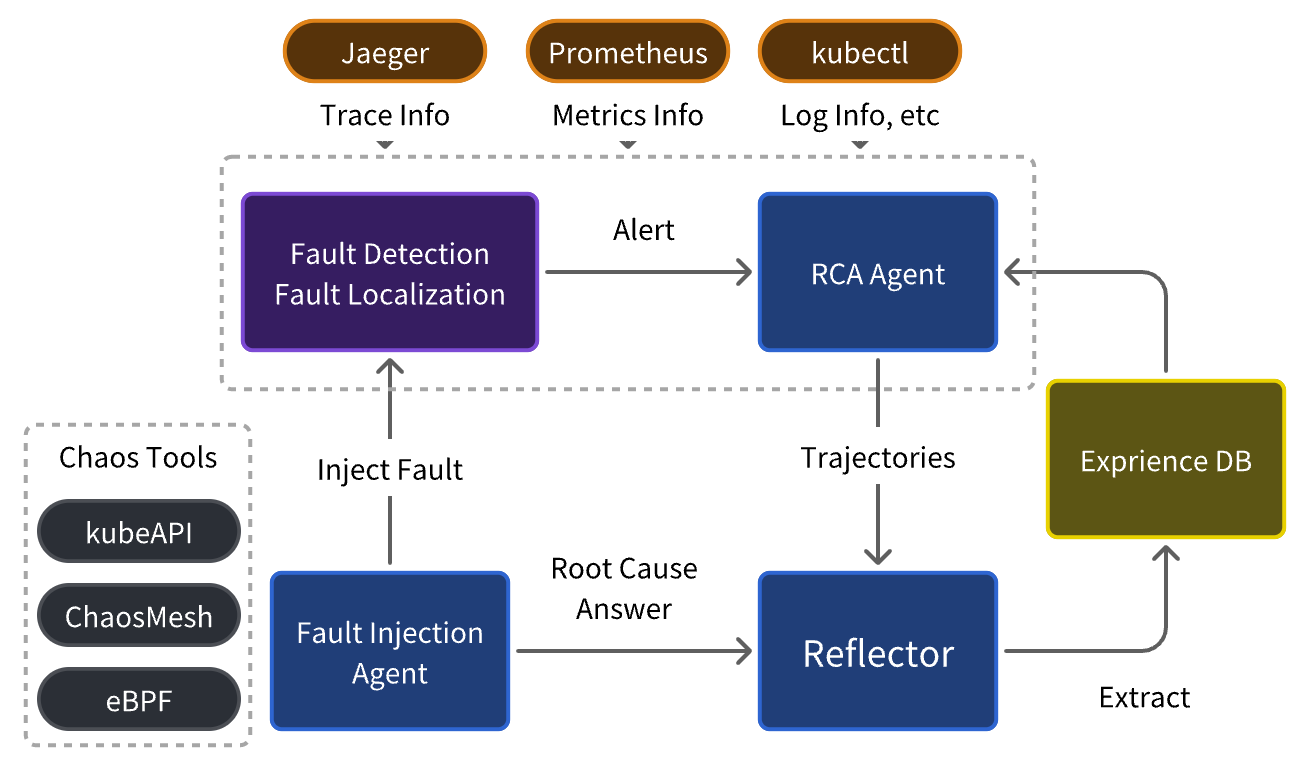
\includegraphics[width=0.6\textwidth]{image/proposal/architecture.png}
        \captionof{figure}{MVP架构} % 使用 \captionof 代替 \caption
        \label{fig:Architecture}
    \end{center}

    现有的在真实云系统环境上评估 LLM Agent 完成 SRE 任务的工作如 ITBench\proposalRef 和 AIOpsLab\proposalRef 等，在传统数据集的基础上实现了集成了云环境部署、故障注入、工作负载生成、遥测数据收集、智能体-云交互和结果评估的互动式框架，为本研究提供了丰富的技术参考、实验环境和数据支持。此外，ChaosEater\proposalRef 等的工作也验证了 LLM Agent 自主进行混沌工程的可行性。综上所述，本研究在技术和资源方面均具备较强的可行性。\proposalRef[4]
}

% 5. 毕业论文（设计）撰写提纲
\thesisOutline{
    （1）绪论。包括：课题研究背景及意义、国内外研究现状。

    （2）系统设计。详细描述所设计的多智能体协作与自适应机制，系统架构及各模块功能。

    （3）实现细节。介绍系统的具体实现方法和关键技术细节，尤其是自主注入故障、自适应机制的实现。

    （4）实验与分析。介绍实验设计、数据收集与分析方法，展示实验结果并进行讨论。

    （5）结语。总结本文所做的工作，阐述其在本研究领域中的意义。
}

% 6. 参考文献
\proposalReferences{
    \begin{enumerate}[label={[\arabic*]}]
        \item Diaz-De-Arcaya J, Torre-Bastida A I, Zárate G, et al. A joint study of the challenges, opportunities, and roadmap of mlops and aiops: A systematic survey[J]. ACM Computing Surveys, 2023, 56(4): 1-30.
        \item 裴丹.AIOps智能运维经验分享[J].深交所, 2022(8):52-57.
        \item Ahmed T, Ghosh S, Bansal C, et al. Recommending root-cause and mitigation steps for cloud incidents using large language models[C]//2023 IEEE/ACM 45th International Conference on Software Engineering (ICSE). IEEE, 2023: 1737-1749.
        \item Zhang W, Guo H, Yang J, et al. mABC: multi-Agent Blockchain-Inspired Collaboration for root cause analysis in micro-services architecture[C]//Findings of the Association for Computational Linguistics: EMNLP 2024. 2024: 4017-4033.
        \item Chen Y, Pan J, Clark J, et al. STRATUS: A Multi-agent System for Autonomous Reliability Engineering of Modern Clouds[J]. In Proceedings of the Thirty-Ninth Annual Conference on Neural Information Processing Systems, 2025.
        \item Tran K T, Dao D, Nguyen M D, et al. Multi-agent collaboration mechanisms: A survey of llms[J]. arXiv preprint arXiv:2501.06322, 2025.
        \item Suzgun M, Yuksekgonul M, Bianchi F, et al. Dynamic cheatsheet: Test-time learning with adaptive memory[J]. arXiv preprint arXiv:2504.07952, 2025.
        \item Zhang Q, Hu C, Upasani S, et al. Agentic context engineering: Evolving contexts for self-improving language models[J]. arXiv preprint arXiv:2510.04618, 2025.
        \item Jha S, Arora R, Watanabe Y, et al. ITBench: Evaluating AI Agents across Diverse Real-World IT Automation Tasks[C]//International Conference on Machine Learning, 2025.
        \item Chen Y, Shetty M, Somashekar G, et al. AIOpsLab: A Holistic Framework to Evaluate AI Agents for Enabling Autonomous Clouds[C]//Eighth Conference on Machine Learning and Systems, 2025.
        \item Kikuta D, Ikeuchi H, Tajiri K. LLM-Powered Fully Automated Chaos Engineering: Towards Enabling Anyone to Build Resilient Software Systems at Low Cost[J]. arXiv preprint arXiv:2511.07865, 2025.
        \item Dong J, Qian K, Zhang P, et al. Evolution of Aegis: Fault Diagnosis for {AI} Model Training Service in Production[C]//22nd USENIX Symposium on Networked Systems Design and Implementation (NSDI 25). 2025: 865-881.
        \item Wang C, Zhang X, Lu R, et al. Towards llm-based failure localization in production-scale networks[C]//Proceedings of the ACM SIGCOMM 2025 Conference. 2025: 496-511.
        \item Chen Y, Xie H, Ma M, et al. Automatic root cause analysis via large language models for cloud incidents[C]//Proceedings of the Nineteenth European Conference on Computer Systems. 2024: 674-688.
        \item Shetty M, Chen Y, Somashekar G, et al. Building ai agents for autonomous clouds: Challenges and design principles[C]//Proceedings of the 2024 ACM Symposium on Cloud Computing. 2024: 99-110.
    \end{enumerate}
}